\documentclass{article}

\usepackage{tikz}
\usepackage{pgfplots}
\usepackage{caption}
\usepackage[export]{adjustbox}

\usetikzlibrary{matrix}

\pgfplotsset{de/.style={
    axis lines=middle,
    xlabel={$D$},
    ylabel={$E$},
    xmin=0, xmax=5,
    ymin=0, ymax=5,
    ticks=none,
    xlabel style={at=(current axis.right of origin), anchor=west},
    ylabel style={at=(current axis.above origin), anchor=south},
}}

\title{Critical Positions: Exploring Depth and Evaluation in Chess}
\date{10 December 2023}

\begin{document}
\maketitle

\section{Introduction}
Aside from strategical ability, the awareness of critical positions is essential for strong chess ability. The evaluation of these positions greatly change with deep calculation. This report aims to investigate how the computer evaluation of the position across different depths can inform us on the importance of studying the position. It will also discuss the logic and implementation to find these critical positions, and how we may study them.

\section{Diagrams}
This report will heavily utilise diagrams to display the evaluation (E) of a position across different depths (D). The evaluation is always relative to who is to move. To simplify discussion, we will say it is White to move. Though depth is discrete, a continous graph will be used for aesthetics.

\begin{center}
    \begin{tikzpicture}
        \begin{axis}[de]
        \addplot [red, domain=0:5, samples=100] {sqrt(x)+1};
        \addplot [green, domain=0:5, samples=100] {x/2+2};
        \end{axis}

        \node [right] at (6.9,3.7) {$M_1$};
    \end{tikzpicture}
\end{center}

We will use a green line to denote the evaluation of the best move in the position. The move that results in this evaluation would likely change across different depths. A red line will be used to denote the evaluation of a certain move. If we are looking at many moves, these may be labelled with $M_n$. If a red $\times$ is used, this indicates that the move was selected on some condition at that depth. Unless otherwise stated, this condition is the best move.

\section{Theory}
We begin by looking at five graphs highlighting features in their most simple and reduced form.

\begin{center}
    
    \begin{tikzpicture}
        \begin{axis}[de, clip=false]
        \addplot [red, domain=0:5, samples=100] {2.5};
        \draw (axis cs:5,2.5) node[red] {$\times$};
        \end{axis}
    \end{tikzpicture}
    \captionof{figure}{}
\end{center}

Figure 1 shows a position with a constant evaluation across the depths. This generally means that intuitive play is sufficient for good play. Though rare, it is possible that there are exceptions.

\begin{center}
    
    \begin{tikzpicture}
        \begin{axis}[de, clip=false]
        \addplot [green, domain=0:5, samples=100] {3/(1 + exp(-5*(x-3.5))) + 1};
        \end{axis}
    \end{tikzpicture}
    \captionof{figure}{}
\end{center}

\begin{center}
    
    \begin{tikzpicture}
        \begin{axis}[de, clip=false]
        \addplot [green, domain=0:5, samples=100] {-3/(1 + exp(-5*(x-3.5))) + 4};
        \end{axis}
    \end{tikzpicture}
    \captionof{figure}{}
\end{center}

Figures 2 and 3 show a position whose evaluation is only evident after calculation. This may represent a range of things in informal terms; the main ones are:
\begin{itemize}
    \item A tactic is present for White
    \item A superior strategy is made possible by a tactic.
    \item The position is strategically winning for White, even though Black's position looks fine.
\end{itemize}
We can imply symmetry on Figure 3.

\begin{center}
    \begin{tikzpicture}
        \begin{axis}[de, clip=false]
        \addplot [red, domain=0:2.5, samples=100] {1.5*exp(-2*(x-2.5)^2) + 2};
        \addplot [red, domain=2.5:5, samples=100] {2.5*exp(-2*(x-2.5)^2) + 1};
        \end{axis}
    \end{tikzpicture}
    \captionof{figure}{}
\end{center}

Figure 4 shows a move which after some depth, appears to be critical. However, after further calculation does not work. These moves are a source of blunder for many. For example, we may see a strong tactic, and experience the confirmation bias as we tell ourselves that it works, and fail to calculate further.

\begin{center}
    \begin{tikzpicture}
        \begin{axis}[de, clip=false]
        \addplot [red, domain=0:2.5, samples=100] {-1.5*exp(-2*(x-2.5)^2) + 2.5};
        \addplot [red, domain=2.5:5, samples=100] {-2.5*exp(-2*(x-2.5)^2) + 3.5};
        \end{axis}
    \end{tikzpicture}
    \captionof{figure}{}
\end{center}

Figure 5 shows move which seems tactically failing, however after the often ignored further calculation, we can see it saves the position.

\section{Testing for Critical Positions}
We now focus on developing logic to find these critical positions.

From Figure 2, we can add the evaluation of the best move at a high depth to produce Figure 6. Note the green line is adjusted for presentability. We can add two values, $\Delta E_0$ and $\Delta E_M$, to denote the change in the best evaluation and red evaluation respectively from some $D$ to a high $D$. In Figure 6, these changes are compared with the evaluation at $D=1$.

\begin{adjustbox}{right=9.9cm}
    \begin{tikzpicture}
    \begin{axis}[de, clip=false]
    \addplot [red, domain=0:5, samples=100] {3/(1 + exp(-5*(x-3.5))) + 1};
    \addplot [green, domain=0:3.5, samples=100] {2.5};
    \addplot [green, domain=3.5:5, samples=100] {3/(1 + exp(-5*(x-3.5))) + 1};
    \draw (axis cs:5,4) node[red] {$\times$};

    \draw[<->] (axis cs:-0.25,2.5) -- (axis cs:-0.25,4) node[midway, left] {$\Delta E_0$};

    \draw[<->] (axis cs:-1,1) -- (axis cs:-1,4) node[midway, left] {$\Delta E_M$};

    \draw[<->] (axis cs:-0.25,1) -- (axis cs:-0.25,2.5) node[midway, left] {$\Delta E_d$};
    \end{axis}

    \end{tikzpicture}
\end{adjustbox}
\captionof{figure}{}

Let $\varepsilon_0$ and $\varepsilon_M$ be thresholds. We now have a few tests for critical positions:
\begin{enumerate}
    \item From $D=1$, $\Delta E_0 > \varepsilon_0$.
    \item From $D=1$, $\Delta E_M > \varepsilon_M$.
    \item $\exists D$ such that from $D$, $\Delta E_0 > \varepsilon_0$.
    \item $\exists D$ such that from $D$, $\Delta E_M > \varepsilon_M$.
\end{enumerate}

We will first investigate whether or not to include comparison across multiple $D$. In computation, (1) and (2) will be much faster than (3) and (4), as fewer evaluations will need to be made. However, (3) and (4) can find critical positions similar to Figure 5, positions that are intuitively evaluated poorly, however deeper calculation shows that they are the best move.

We also have to decide whether to use $\varepsilon_0$ or $\varepsilon_M$. Defining a critical position by $\varepsilon_0$ indicates that calculating and executing the best move makes White much better off. Setting a high $\varepsilon_0$ can filter out some positional lines. In contrast, a high $\varepsilon_M$ can be used to positions whose best move should not be played without full calculation. This is useful to find more moves that are more ``risky''. 

Figure 6 also has marked $\Delta E_d$ the difference between the two evaluation at some $D$. Let $\delta$ be some threshold to indicate a large difference in evaluation. We can illustrate the type of position by whether certain thresholds were exceeded in the following table:

\begin{center}
    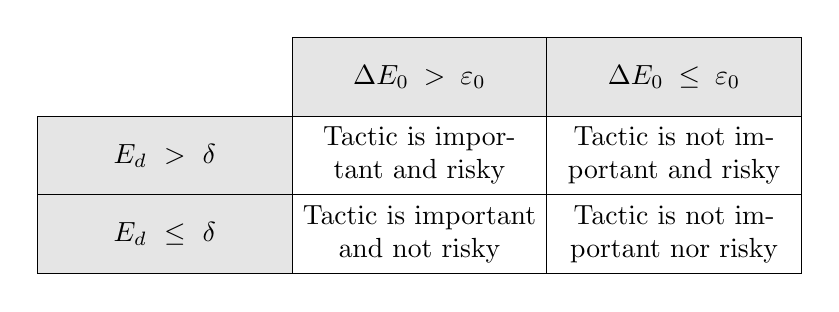
\begin{tikzpicture}
    \matrix (mytable) [
      matrix of nodes,
      nodes in empty cells,
      nodes={draw, minimum size=1cm, anchor=center, text width=3cm,align=center},
      column sep=-\pgflinewidth,
      row sep=-\pgflinewidth,
      row 1/.style={nodes={fill=gray!20}},
      column 1/.style={nodes={fill=gray!20}},
      row 1 column 1/.style={nodes={fill=none, text opacity=0, draw=none}},
    ] {
       & $\Delta E_0 > \varepsilon_0$ & $\Delta E_0 \leq \varepsilon_0$ \\
       $E_d > \delta$ & Tactic is important and risky & Tactic is not important and risky \\
       $E_d \leq \delta$ & Tactic is important and not risky & Tactic is not important nor risky \\
    };
  \end{tikzpicture}
\end{center}

We should prioritise studying risky and important tactics, as those will have the greatest impact when they do arise. We should note that $\Delta E_0$ is not the only measurement of ``risk''; for example, a high $D$ when the threshold is exceeded could also be risky, as the longer line must be calculated increasing the chance of mistake. Risk is subjective and the familiarity of the position is a factor.


\begin{adjustbox}{right=9.9cm}
    \begin{tikzpicture}
        \begin{axis}[de, clip=false]
        \addplot [red, domain=0:5, samples=100] {-3/(1 + exp(-5*(x-3.5))) + 4};
        \addplot [green, domain=0:2, samples=100] {4};
        \addplot [green, domain=2:5, samples=100] {-1/(1 + exp(-5*(x-3.5))) + 4};
        \draw (axis cs:0,4) node[red] {$\times$};

        \draw[<->] (axis cs:-0.25,3) -- (axis cs:-0.25,4) node[midway, left] {$\Delta E_0$};

        \draw[<->] (axis cs:-1,1) -- (axis cs:-1,4) node[midway, left] {$\Delta E_M$};

        \draw[<->] (axis cs:-0.25,1) -- (axis cs:-0.25,3) node[midway, left] {$\Delta E_d$};
        \end{axis}
    \end{tikzpicture}
\end{adjustbox}
\captionof{figure}{}

Figure 7 is the opposite of Figure 6. Instead to the inability to seize an oppourtunity at low depth, we instead play an intuitive move that is a mistake.

We do not have build another program and set of logic for Figure 7, as it is identical to Figure 6 but from the opponent's perspective.

True expertise in chess is not only the ability to seize these opportunities, and avoiding intuitive moves that allow the opponent to seize an opportunity. It is also the ability to identify these positions before they arise. This can only be done through a careful investigation into piece placement and pawn structure, and relating them unintuitive ideas.

\end{document}